\subsection{Extended sliding modes control techniques}\label{S02-4}

As seen in subsections 2.1 and 2.2, it's very convenient to use redundant coordinates to perform parallel mechanism dynamic modeling. 
The aim of this subsection it to propose a control law for systems described by redundant coordinates.

Let $\ssM$ be a multibody mechanical system whose mathematical model is given 
by equations~(\ref{eq:02-105B},~\ref{eq:02-112B}).
For the sake of brevity, no system index $n$ will be used in this subsection.
Suppose that each $\mf$ is an affine function of the control inputs $u_{k}$
in which the coefficients of the $u_{k}$ may depend on the instantaneous
configuration of the system.
Suppose additionally that that all the $\mA$ are independent
of the quasi-velocities $p_{j}$ and all the $\mM$, $\mg$, $\mA$ and $\mb$ 
are independent of the $u_{k}$.
Under these conditions, matrices $\mC$ will not depend on 
any quasi-velocity, $\md$ can be expressed as an affine function of the control inputs 
and $\mc$ is independent of them.
Considering that the number of control inputs in $\ssM$ is
exactly equal to the number of degrees of freedom of $\ssM$, 
there exists a particular matrix $\mC(t,\mq)$ such that:
\begin{equation} \label{eq:InverseDynamics}
\mu = \mC^\msT(t,\mq) \Big( \mM (t, \mq) \, \dot{\mp} + \mw(t,\mq,\mp) + \mz(t,\mq) \Big)
\end{equation}
In equation \eqref{eq:InverseDynamics}, $\mw$ is a column-vector representing terms of generalized force 
or generalized gyroscopic inertia force which are linear or bilinear with respect to quasi-velocities 
and $\mz$ stems from terms that are independent of these variables.

From the control perspective, it is convenient to work with mathematical models in which $\mp = \dot \mq$, 
in order to have a position feedback control.
Thus, based on equations \eqref{eq:InverseDynamics} and \eqref{eq:02-201A}, consider that 
the mathematical model of $\ssM$ is given by the following equations:
\begin{equation} \label{eq:MechanicalSystem}
\begin{cases}
\mC^\msT (t, \mq) \Big( \mM (t, \mq) \, \ddot{\mq} + \mw (t, \mq, \dot{\mq}) + \mz (t, \mq) \Big) = \mu \\
\mA (t, \mq) \, \ddot{\mq} + \mb (t, \mq, \dot{\mq}) = \mzr
\end{cases}
\end{equation}
Rewriting in a compact matrix form:
\begin{equation} \label{eq:MechanicalSystemMatrix}
\begin{bmatrix}
\mC^\msT \mM \\
\mA
\end{bmatrix}
\ddot{\mq}
=
\begin{bmatrix}
\mu - \mC^\msT(\mw + \mz) \\
-\mb
\end{bmatrix}
\end{equation}
The desired control law should satisfy, in closed loop, the condition $ \ddot{\mq} = \mv $, with $\mv$ being 
a control input column-matrix. 
Thus, the following control law should be used:
\begin{equation} \label{eq:ControlLawV}
\mu = \mC^\msT ( \mM \, \mv + \mw + \mz )
\end{equation}
Once $ \ddot{\mq} = \mv $, and $\ddot{\mq}$ has to satisfy constraint equations, $\mv$ must respect the same restrictions, i.e.:
\begin{equation} \label{eq:ControlLawVRestriction}
\mA \, \mv + \mb = \mzr
\end{equation}
Applying the control law \eqref{eq:ControlLawV} and the 
rectritions \eqref{eq:ControlLawVRestriction} in \eqref{eq:MechanicalSystemMatrix}: 
\begin{align*}
&	\begin{bmatrix}
	\mC^\msT \, \mM \\
	\mA
	\end{bmatrix}
	\ddot{\mq}
	=
	\begin{bmatrix}
	\mC^\msT ( \mM \, \mv + \mw + \mz ) - \mC^\msT(\mw + \mz) \\
	\mA \, \mv
	\end{bmatrix}
	=
	\begin{bmatrix}
	\mC^\msT  \, \mM \, \mv \\
	\mA \, \mv
	\end{bmatrix}
	=
	\begin{bmatrix}
	\mC^\msT \mM \\
	\mA
	\end{bmatrix}
	\mv 
\end{align*}
Once the matrix $\begin{bmatrix} \mC^\msT \, \mM \\ \mA \end{bmatrix}$ is non-singular:
\begin{equation} \label{eq:ClosedLoopV}
\ddot{\mq} = \mv
\end{equation}

Let $\mv'$ be given by the sliding modes control law:
\begin{equation} \label{eq:SMControlowLasV1'}
\mv' = \ddot{\mq}^\sdia + \lambda \dot{\me} + k \sign (\dot{\me} + \lambda \me)
\end{equation}
Being $ \me = \mq^\sdia - \mq $ the error signal and $\mq^\sdia$ the reference signal. If there were no retrictions, it could be stated that $ \mv = \mv' $, and:
\begin{align*}
	\ddot{\mq} = \mv \qquad \Rightarrow \qquad \ddot{\me} + \lambda \dot{\me} + k \sign (\dot{\me} + \lambda \me) = \mzr 
	\qquad \Leftrightarrow \qquad \dot{\ms} = - k \sign(\ms)
\end{align*}
This would ensure that $\me \rightarrow 0$ when $t \rightarrow \infty$ for any initial condition, as seen in the last subsection. 

Once $\mv$ can not be freely set as $\mv'$, the following optimization problem is proposed:
\begin{align} \label{eq:Optimization}
& 	\min_{\mv} \quad (\mv - \mv')^\msT \, \mM \, (\mv - \mv') 
	\qquad \text{s.t.} \qquad \mA \, \mv + \mb = \mzr
\end{align}
As $\mM$ is positive-semidefinite, then $(\mv - \mv')^\msT \, \mM \, (\mv - \mv') \geq 0 $ for any $\mv$.

Applying the method of Lagrange undetermined multipliers, it can be stated that this
optimization problem is equivalent to minimize with respect to $\mv$ and $\mlambda$
the following functional:
\begin{equation}
L = (\mv - \mv')^\msT \, \mM \, (\mv - \mv') + (\mA \mv + \mb)^\msT \, \mlambda 
\end{equation}
To solve the problem, the Lagrangian function must be stationary. Thus:
\begin{align}
 	\dl L = 0 \qquad &\Rightarrow \qquad  
 	\dl \mv^\msT \mM (\mv - \mv') + (\mv - \mv')^\msT \mM \dl \mv + (\mA \dl \mv)^\msT \mlambda 
		+ (\mA \mv + \mb)^\msT \dl \mlambda = 0 
	\nonumber \\	
& 	\Rightarrow \qquad
	\dl \mv^\msT \left( (\mM + \mM^\msT)(\mv - \mv') + \mA^\msT \mlambda \right) + \dl \mlambda^\msT (\mA \mv + \mb) = 0 
\end{align}
Once $\mM$ is symmetric and $\dl \mv$ and $\dl \mlambda$ are arbitrary:
\begin{equation} \label{eq:OptimizationSol}
\begin{cases}
2 \, \mM \, (\mv - \mv') + \mA^\msT \mlambda = \mzr \\
\mA \, \mv + \mb = \mzr
\end{cases}
\end{equation}
Considering that $\mC$ is an orthogonal complement of $\mA$, pre-multiplying the first equation of 
\eqref{eq:OptimizationSol} by $\mC^\msT$ leads to:
\begin{align}
& 	2 \, \mC^\msT \, \mM (\mv - \mv') + \mC^\msT \, \mA^\msT \mlambda = \mzr 
	\qquad 	\Rightarrow \qquad \mC^\msT \, \mM (\mv - \mv')  = \mzr 
	\qquad \therefore \qquad \mC^\msT \, \mM \, \mv  = \mC^\msT \, \mM \, \mv'
	\label{eq:OptimizationSol2}
\end{align}
Thus, the control law that makes the closed loop system as close as possible of $\ddot{\mq} = \mv'$, 
according to the optimization criterion adopted, is:
\begin{equation} \label{eq:ControlLawFinal}
\mu = \mC^\msT ( \mM \, \mv' + \mw + \mz )
\end{equation}

\begin{figure}[H]
	\centering
	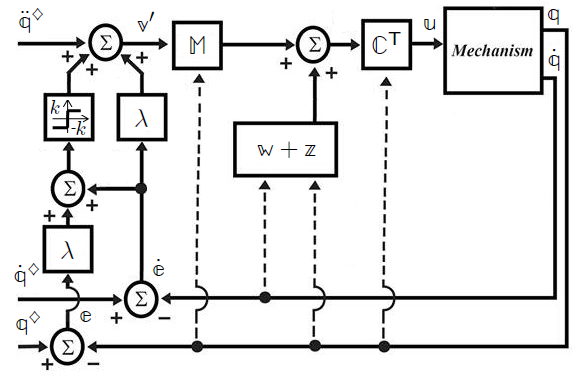
\includegraphics[scale=0.75]{ControlDiagram.png}
	\caption{Extended sliding modes control loop}
	\label{ControlDiagram}
\end{figure}

